% Ivan Hip / 2019-05-08

\documentclass{beamer}
\usetheme{Frankfurt}

% Ivan Hip / 2019-05-08
% iskustvo je pokazalo da kod korištenja Beamera treba učitati ove pakete

\usepackage[croatian]{babel}
\usepackage[utf8]{inputenc}
\usepackage[T1]{fontenc}
\usepackage{lmodern}

\hypersetup{unicode = true}

% Ivan Hip / 2019-05-08
% jedinstveni naslovni slajd za prezentacije

\newcommand{\naslov}[1]{
	\title{#1}
	\author{Ivan Hip}
	\institute{Geotehnički fakultet, Sveučilište u Zagrebu}
	\date{
\includegraphics[width=0.15\textwidth]{../CC-by-sa.pdf}}
} % \newcommand

\newcommand{\naslovnislajd}{
	\begin{frame}
		\titlepage
	\end{frame}
} % \newcommand

\naslov{Tečenje u otvorenim koritima}

\begin{document}
\naslovnislajd

\section{Tečenje u otvorenim koritima}
\begin{frame}{Tečenje u otvorenim koritima}

\begin{itemize}
\item u literaturi na engleskom jeziku: \alert{open-channel flow}
\item treba razlikovati engleske riječi \alert{channel} i \alert{canal}
--- \emph{channel} može biti \emph{artificial channel}, ali i \emph{natural
channel}, dakle prirodno nastali vodeni put koji u našem jeziku obično
nazivamo korito (rijeke ili potoka), dok je engleski \emph{canal}
upravo ono što je kanal i u hrvatskom jeziku, tj. umjetno stvoreni
vodeni put
\item poseban je slučaj kada se riječ\emph{ channel} odnosi na pojas mora
između dva komada kopna --- tada se prevodi kao kanal (kanal La Manche
ili Zadarski kanal)
\item u literaturi na hrvatskom jeziku koristi se i naziv \emph{tečenje
sa slobodnim vodnim licem} --- dakle, uvijek postoji slobodna površina
tekućine (uglavnom vode), nad kojom je (najčešće) atmosferski tlak
\end{itemize}
\end{frame}

\begin{frame}{Nema razlike tlakova}

\begin{itemize}
\item činjenica da je nad čitavom površinom tekućine isti tlak isključuje
mogućnost tečenja zbog razlike tlakova (što je bio osnovni pokretački
mehanizam u cijevima potpuno ispunjenim tekućinom)
\item preostaje samo sila teža, tj. voda teče prema dolje :-)
\item izgleda jednostavnije od tečenja u cijevima, ali nije: ključna razlika
je što se u otvorenim koritima može mijenjati razina tekućine ---
to dovodi do promjene površine presjeka i omočenog oboda, a time se
mijenja i protok i otpor uslijed djelovanja viskoznog trenja ---
sve postaje znatno složenije!
\item cijev koja nije u potpunosti ispunjena tekućinom zapravo je specijalni
slučaj tečenja u otvorenim koritima --- u takvoj cijevi nije moguće
postići razliku tlakova, a razina tekućine može se slobodno mijenjati
\end{itemize}
\end{frame}

\begin{frame}{Tečenje u otvorenim koritima uglavnom je turbulentno}

\begin{itemize}
\item kod tečenja u otvorenim koritima obično se radi o tečenju vode u prirodnim
ili umjetnim koritima, dakle potocima, rijekama i kanalima kojima
je tipični promjer od jednog pa do više desetaka metara
\item tipična brzina tečenja je od nekoliko centimetara do nekoliko metara
u sekundi
\item kada se te tipične vrijednosti za $D_{h}$ i $\bar{v}$ zajedno s
kinematičkom viskoznošću vode koja je oko $10^{-6}m^{2}s^{-1}$ uvrste
u izraz za Reynoldsov broj
\[
\mathrm{Re}=\frac{\bar{v}D_{h}}{\nu}=\frac{1ms^{-1}\cdot10m}{10^{-6}m^{2}s^{-1}}=10^{7}
\]
jasno je da se dobivaju vrijednosti koje su duboko u turbulentnom
režimu tečenja
\end{itemize}
\end{frame}

\section{Energijska jednadžba}
\begin{frame}{Energijska jednadžba za tečenje u otvorenim koritima}

\begin{itemize}
\item za tečenje u cijevima energijska jednadžba je
\[
\frac{p_{{\scriptscriptstyle A}}}{\rho g}+z_{{\scriptscriptstyle A}}+\alpha_{{\scriptscriptstyle A}}\frac{\bar{v}_{{\scriptscriptstyle A}}^{2}}{2g}+h_{P}-h_{T}=\frac{p_{{\scriptscriptstyle B}}}{\rho g}+z_{{\scriptscriptstyle B}}+\alpha_{{\scriptscriptstyle B}}\frac{\bar{v}_{{\scriptscriptstyle B}}^{2}}{2g}+h_{F}
\]
\item pošto kod tečenja u otvorenim koritima nije moguće uspostaviti razliku
tlakova, nije moguće ni pumpanje pa član $h_{P}$ (visina dobave pumpe)
nema smisla
\item što se tiče člana $h_{T}$ (pad visine na turbini) on bi imao smisla
(nesumnjivo je moguće iskoristiti dio mehaničke energije tekućine
koja teče u otvorenom koritu --- na primjer vodenica), ali ćemo ga
zbog jednostavnosti izostaviti
\item s obzirom da smo duboko u turbulentnom režimu tečenja uzimamo da su
Coriolisovi koeficijenti $\alpha_{_{A}},\alpha_{_{B}}$ jednaki jedinici 
\end{itemize}
\end{frame}

\begin{frame}{Što znači tlačna visina na presjeku?}

\begin{itemize}
\item konačno, opet radi jednostavnosti, ograničit ćemo se samo na linijski
gubitak duž korita, dakle umjesto $h_{F}$ samo $h_{f}$
\[
\frac{p_{{\scriptscriptstyle A}}}{\rho g}+z_{{\scriptscriptstyle A}}+\frac{\bar{v}_{{\scriptscriptstyle A}}^{2}}{2g}=\frac{p_{{\scriptscriptstyle B}}}{\rho g}+z_{{\scriptscriptstyle B}}+\frac{\bar{v}_{{\scriptscriptstyle B}}^{2}}{2g}+h_{f}
\]
\item sa srednjim brzinama $\bar{v}_{_{A}}$ i $\bar{v}_{_{B}}$ nema problema,
one se mogu jednoznačno definirati (i, barem u principu, točno izmjeriti)
kao protok kroz površinu presjeka
\item za geodetske visine $z_{_{A}}$ i $z_{_{B}}$ dogovorno se uzimaju
geodetske visine dna, tj. najniže točke presjeka $A$ i $B$
\end{itemize}
\begin{block}{}
Postavlja se pitanje što točno znači tlačna visina na presjeku ---
i da li ju je uopće moguće precizno definirati? 
\end{block}
\end{frame}

\begin{frame}{Dubina toka}

\begin{center}
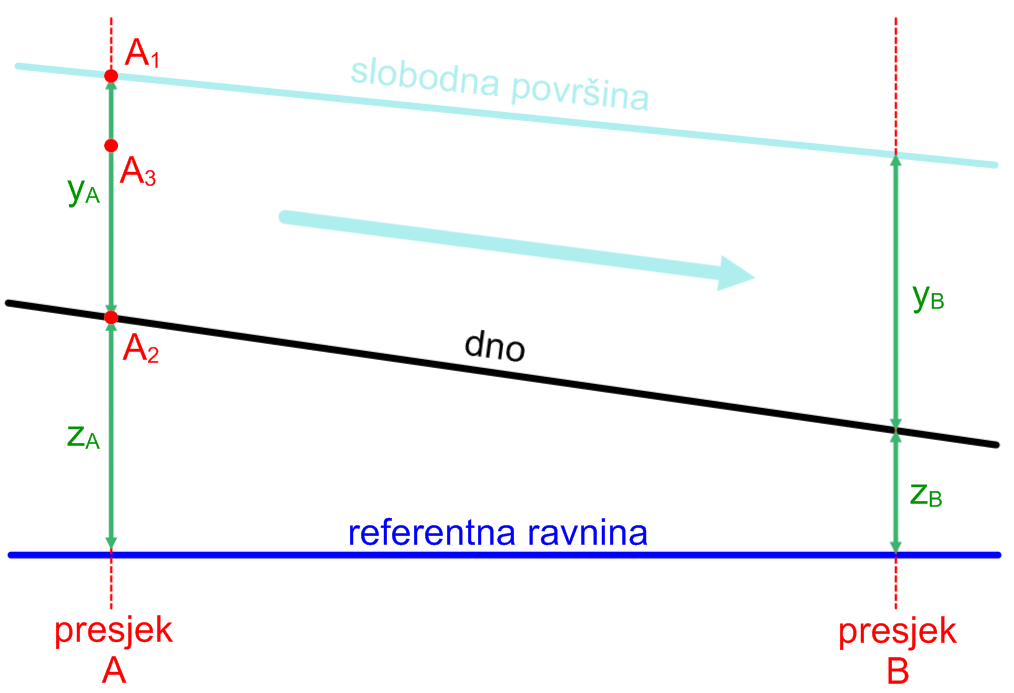
\includegraphics[height=0.5\paperheight]{slike/MF-10-slika1.PNG}
\par\end{center}
\begin{itemize}
\item $y_{_{A}}$ i $y_{_{B}}$ su dubine (udaljenosti od slobodne površine
do dna)
\item podrazumijevamo da se geometrija presjeka ne mijenja!
\end{itemize}
\end{frame}

\begin{frame}{Tri točke na presjeku}

Računamo ukupnu energijsku visinu za tri točke $A_{1}$, $A_{2}$
i $A_{3}$ koje se nalaze na presjeku $A$:
\begin{itemize}
\item točka $A_{1}$ je na slobodnoj površini tekućine, tlak je atmosferski
$p_{_{A_{1}}}=p_{_{a}}$, a geodetska visina $z_{_{A_{1}}}=z_{_{A}}+y_{_{A}}$,
dakle
\[
E_{_{A_{1}}}=\frac{p_{_{a}}}{\rho g}+z_{_{A}}+y_{_{A}}+\frac{\bar{v}_{_{A}}^{2}}{2g}
\]
\item točka $A_{2}$ je na dnu korita, $z_{_{A_{2}}}=z_{_{A}}$, a tlak
je suma atmosferskog tlaka i tlaka uslijed visine stupca tekućine,
dakle $p_{_{A_{2}}}=p_{_{a}}+\rho gy_{_{A}}$ pa je 
\[
E_{_{A_{2}}}=\frac{p_{_{a}}+\rho gy_{_{A}}}{\rho g}+z_{_{A}}+\frac{\bar{v}_{_{A}}^{2}}{2g}=\frac{p_{_{a}}}{\rho g}+y_{_{A}}+z_{_{A}}+\frac{\bar{v}_{_{A}}^{2}}{2g}
\]
\end{itemize}
\end{frame}

\begin{frame}{Ukupna energijska visina presjeka}

\begin{itemize}
\item točka $A_{3}$ je na proizvoljnoj dubini $y_{_{A_{3}}}<y_{_{A}}$,
tlak je suma atmosferskog tlaka i tlaka uslijed visine stupca tekućine
$p_{_{A_{3}}}=p_{_{a}}+\rho gy_{_{A_{3}}}$, a geodetska visina $z_{_{A_{3}}}=z_{_{A}}+y_{_{A}}-y_{_{A_{3}}}$,
što sve zajedno daje
\[
E_{_{A_{3}}}=\frac{p_{_{a}}+\rho gy_{_{A_{3}}}}{\rho g}+z_{_{A}}+y_{_{A}}-y_{_{A_{3}}}+\frac{\bar{v}_{_{A}}^{2}}{2g}=\frac{p_{_{a}}}{\rho g}+z_{_{A}}+y_{_{A}}+\frac{\bar{v}_{_{A}}^{2}}{2g}
\]
\end{itemize}
\begin{block}{}
Za sve tri točke na presjeku dobili smo istu ukupnu energijsku visinu
pa možemo jednoznačno definirati \alert{ukupnu energijsku visinu presjeka}\emph{
\[
E_{_{A}}\equiv\frac{p_{_{a}}}{\rho g}+y_{_{A}}+z_{_{A}}+\frac{\bar{v}_{_{A}}^{2}}{2g}
\]
}
\end{block}
\end{frame}

\begin{frame}{Energijska jednadžba za tečenje u otvorenim koritima}

\begin{itemize}
\item izjednačavanjem ukupnih energijskih visina na presjecima $A$ i $B$
dobivamo
\[
\frac{p_{_{a}}}{\rho g}+y_{_{A}}+z_{{\scriptscriptstyle A}}+\frac{\bar{v}_{{\scriptscriptstyle A}}^{2}}{2g}=\frac{p_{_{a}}}{\rho g}+y_{_{B}}+z_{{\scriptscriptstyle B}}+\frac{\bar{v}_{{\scriptscriptstyle B}}^{2}}{2g}+h_{f}
\]
\item očito, tlačne visine zbog atmosferskog tlaka se krate i dobivamo energijsku
jednadžbu za tečenje u otvorenim koritima
\end{itemize}
\begin{alertblock}{Energijska jednadžba za tečenje u otvorenim koritima}
\[
y_{_{A}}+z_{{\scriptscriptstyle A}}+\frac{\bar{v}_{{\scriptscriptstyle A}}^{2}}{2g}=y_{_{B}}+z_{{\scriptscriptstyle B}}+\frac{\bar{v}_{{\scriptscriptstyle B}}^{2}}{2g}+h_{f}
\]
\end{alertblock}
\begin{itemize}
\item dubine $y_{_{A}}$ i $y_{_{B}}$ imaju ulogu tlačnih visina
\end{itemize}
\end{frame}

\section{Jednoliko tečenje}
\begin{frame}{Jednoliko tečenje (engl. \emph{uniform flow})}

\begin{itemize}
\item \alert{jednoliko tečenje} podrazumijeva da se duž korita dubina
toka ne mijenja, tj. da za svaka dva presjeka $A$ i $B$ vrijedi
$y_{_{A}}=y_{_{B}}$
\item kako smo pretpostavili i da se geometrija presjeka ne mijenja, ista
dubina toka znači i istu površinu presjeka što za konstantni protok
znači da je $\bar{v}_{_{A}}=\bar{v}_{_{B}}$, tj. ne mijenja se ni
dubina, ni srednja brzina tečenja
\item u tom slučaju energijska jednadžba postaje
\[
z_{_{A}}-z_{_{B}}=h_{f}=\lambda\frac{L}{D_{h}}\frac{\bar{v}^{2}}{2g}
\]
i iz nje je moguće odrediti srednju brzinu, a time i protok, ukoliko
je poznata geometrija korita, uključujući i visinsku razliku $\Delta z=z_{_{A}}-z_{_{B}}$
između presjeka $A$ i $B$
\end{itemize}
\end{frame}

\begin{frame}{Nagib dna}

\begin{itemize}
\item uvažavajući da je $D_{h}\equiv4R_{h}$ iz energijske jednadžbe slijedi
\[
\bar{v}^{2}=\frac{2g}{\lambda}4R_{h}\frac{z_{_{A}}-z_{_{B}}}{L}=\frac{8g}{\lambda}R_{h}I
\]
pri čemu je $I$ \alert{nagib dna} (engl. \emph{bottom slope}) koji
je definiran kao
\[
I\equiv\frac{z_{_{A}}-z_{_{B}}}{L}=\frac{\Delta z}{L}
\]
\end{itemize}
\begin{block}{Srednja brzina kod jednolikog tečenja u otvorenom koritu}
\[
\bar{v}=\sqrt{\frac{8g}{\lambda}}\sqrt{R_{h}I}
\]
\end{block}
\begin{itemize}
\item ova formula doista se može koristiti u praksi --- kroz koeficijent
otpora trenja $\lambda$ u proračun ulazi i hrapavost korita
\end{itemize}
\end{frame}

\begin{frame}{Chezyjeva formula}

\begin{itemize}
\item u praksi se još uvijek koriste i ``tradicionalne'' formule
\item da srednja brzina (protok) kod jednolikog tečenja u otvorenom koritu
ovisi o korijenu iz hidrauličkog polumjera i nagiba dna bilo je poznato
francuskom inženjeru Chezyju još krajem 18. stoljeća!
\item \alert{Chezyjeva formula} iz 1776. godine je
\[
\bar{v}=C\sqrt{R_{h}I}
\]
pri čemu je $C$ Chezyjev koeficijent
\item tijekom 19. stoljeća mnogi su se inženjeri bavili problemom kako odrediti
$C$, a još danas se u praksi često koristi formula irskog inženjera
Manninga iz 1891. godine (slična je i formula njemačkog inženjera
Stricklera iz 1923. godine)
\end{itemize}
\end{frame}

\begin{frame}{Manningova formula}

\begin{itemize}
\item Manning je unaprijedio Chezyjevu formulu uzevši da je $C=R_{h}^{1/6}/n$
gdje je $n$ bezdimenzionalni koeficijent koji se danas naziva \alert{Manningov koeficijent hrapavosti}
i ovisi o vrsti, tj. hrapavosti korita --- u praksi se uzima iz tablica
\end{itemize}
\begin{alertblock}{Manningova formula}
\[
\bar{v}=\frac{1}{n}R_{h}^{2/3}I^{1/2}
\]
\end{alertblock}
\begin{itemize}
\item vrijednosti nagiba dna su u stvarnosti izuzetno male --- primjer
rijeke Mississippi: izvor je na 448 metara nadmorske visine, a do
ušća u Atlantski ocean ima 3782 kilometra, što daje (srednji) nagib
dna $I=0,000118$
\end{itemize}
\end{frame}

\section{Mirni i siloviti tok}
\begin{frame}{Specifična energija presjeka}

\begin{itemize}
\item glavno svojstvo tečenja u otvorenim koritima --- da se razina (dubina)
tekućine može slobodno mijenjati --- ima za posljedicu čitav niz
zanimljivih efekata od kojih je možda najzanimljivija pojava \alert{mirnog}
i \alert{silovitog} tečenja
\item pokazat će se da dubina tečenja nije jednoznačno određena čak ni kada
su istovremeno zadani protok i specifična energija tekućine!
\item s obzirom da se geodetska visina dna praktički ne mijenja (tj. mijenja
se erozijskim procesima u vrlo velikim vremenskim razdobljima) dovoljno
je analizirati takozvanu \alert{specifičnu energiju presjeka}
\[
E_{S}=y+\frac{\bar{v}^{2}}{2g}=y+\frac{1}{2g}\frac{Q^{2}}{S^{2}}
\]
\end{itemize}
\end{frame}

\begin{frame}{Korito pravokutnog presjeka}

\begin{itemize}
\item ako se ne mijenja geometrija korita, jasno je da će promjena dubine
također dovesti do promjene površine presjeka, tj. jasno je da je
površina presjeka funkcija dubine: $S=S(y)$
\item analizirat ćemo najjednostavniji slučaj: korito (kanal) pravokutnog
presjeka širine $B=konst.$ kojem je površina presjeka $S(y)=By$,
a specifična energija presjeka
\[
E_{S}=y+\frac{\bar{v}^{2}}{2g}=y+\frac{1}{2g}\frac{Q^{2}}{S(y)^{2}}=y+\frac{1}{2g}\frac{Q^{2}}{B^{2}y^{2}}
\]
\item za zadani protok $Q=konst.$ specifična energija presjeka je funkcija
samo jedne varijable --- dubine $y$
\[
E_{S}(y)=y+\frac{1}{2g}\frac{Q^{2}}{B^{2}y^{2}}
\]
\end{itemize}
\end{frame}

\begin{frame}{Asimptote}

Ako analiziramo tok funkcije
\[
E_{S}(y)=y+\frac{1}{2g}\frac{Q^{2}}{B^{2}y^{2}}
\]

\begin{itemize}
\item za velike dubine tečenja $y\gg1$ specifična energija presjeka se
asimptotski približava pravcu
\[
E_{S}(y\gg1)\simeq y
\]
\item kod malih dubina, kad je $y\ll1$ asimptotski se približava krivulji
\[
E_{S}(y\ll1)\simeq\frac{1}{2g}\frac{Q^{2}}{B^{2}y^{2}}
\]
\end{itemize}
\end{frame}

\begin{frame}{Ovisnost specifične energije presjeka o dubini}

\begin{center}
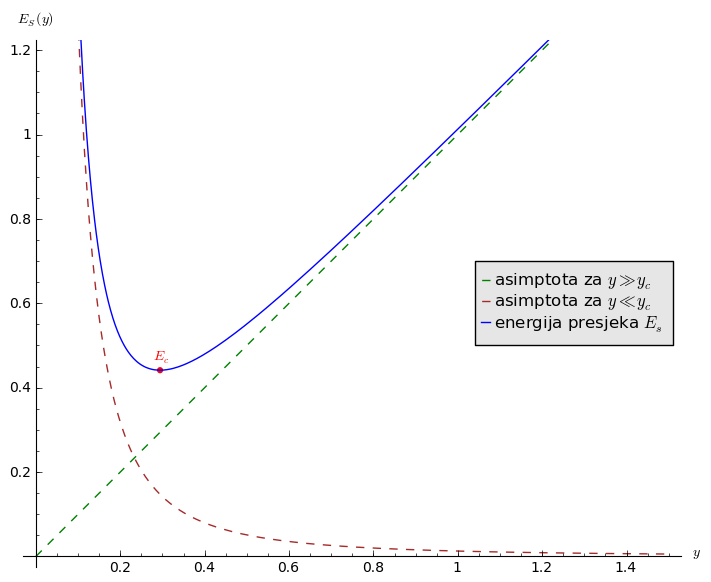
\includegraphics[height=0.7\paperheight]{slike/MF-10-kriticna-energija}
\par\end{center}

\end{frame}

\begin{frame}{Rješenja za zadani protok $Q=konst.$}

\begin{itemize}
\item za zadani protok $Q=konst.$ uvijek postoji minimum specifične energije
presjeka, takozvana \alert{kritična energija}\emph{ $E_{c}$}
\item vidljivo je da za energiju manju od kritične ne postoji realno rješenje
--- dakle, potrebna je specifična energija presjeka $E_{S}(y)\geq E_{c}$
da bi se protok $Q$ uopće mogao realizirati!
\item ukoliko je $E_{S}(y)=E_{c}$ tada je dubina tečenja jednoznačno određena
i to je \alert{kritična dubina}\emph{ $y_{c}$}
\item kad je energija blizu kritične, mala promjena energije dovodi do velike
promjene dubine --- takve nagle promjene mogu dovesti do oštećenja
hidrotehničkih objekata pa otuda i dolaze nazivi \emph{kritična energije}
i \emph{kritična dubina}
\end{itemize}
\end{frame}

\begin{frame}{Određivanje kritične dubine}

\begin{itemize}
\item kritična dubina $y_{c}$ je minimum funkcije $E_{S}(y)$ i može se
odrediti iz uvjeta
\[
\frac{dE_{S}}{dy}=0
\]
\item derivacija specifične energije presjeka po $y$ je
\[
\frac{dE_{S}}{dy}=\frac{d}{dy}\left(y+\frac{1}{2g}\frac{Q^{2}}{B^{2}y^{2}}\right)=1+\frac{Q^{2}}{2gB^{2}}(-2)\frac{1}{y^{3}}=1-\frac{Q^{2}}{gB^{2}}\frac{1}{y^{3}}
\]
\item pa slijedi
\[
1-\frac{Q^{2}}{gB^{2}}\frac{1}{y_{c}^{3}}=0\quad\Rightarrow\quad y_{c}^{3}=\frac{Q^{2}}{gB^{2}}\quad\Rightarrow\quad y_{c}=\sqrt[3]{\frac{Q^{2}}{gB^{2}}}
\]
\end{itemize}
\end{frame}

\begin{frame}{Energija presjeka veća od kritične energije $\Rightarrow$ dva rješenja!}

\begin{center}
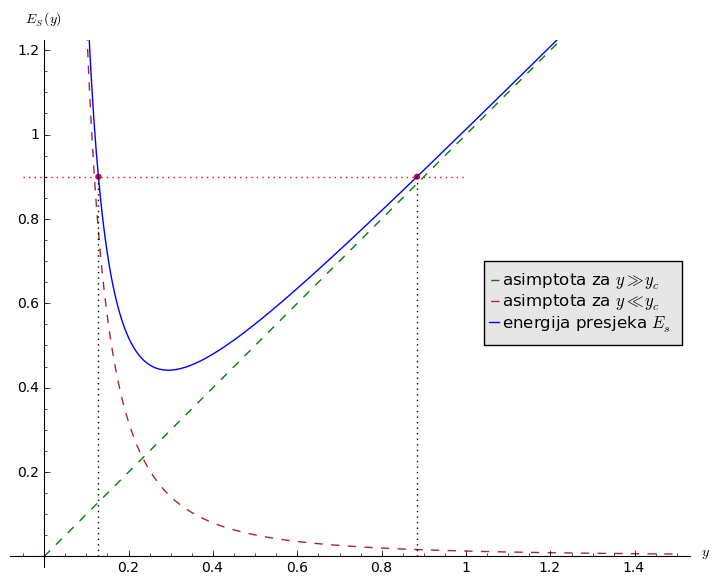
\includegraphics[height=0.7\paperheight]{slike/MF-10-mirni-i-siloviti-tok}
\par\end{center}

\end{frame}

\begin{frame}{Alternativne dubine}

\begin{itemize}
\item ukoliko je na raspolaganju više energije od kritične, tj. $E_{S}(y)>E_{c}$
iz grafikona je vidljivo da postoje dva rješenja, takozvane \alert{alternativne dubine}
\item dva formalna, matematička, rješenja doista su realizirana u stvarnosti!
\item zbog relacije 
\[
\bar{v}=\frac{Q}{S}=\frac{Q}{By}=\bar{v}(y)
\]
očito da za neki zadani protok $Q$ mala dubina tečenja znači veliku
srednju brzinu i obrnuto, velika dubina tečenja znači manju srednju
brzinu, tj. sporije tečenje
\end{itemize}
\end{frame}

\begin{frame}{Mirni i siloviti tok}

\begin{block}{Mirni i siloviti tok}

Za zadani protok $Q$ i zadanu specifičnu energiju $E_{S}>E_{c}$
moguće su dvije dubine tečenja, jedna manja, a druga veća od kritične
dubine:

\begin{itemize}
\item za dubinu manju od kritične karakteristična je veća brzina toka pa
otuda naziv \alert{siloviti tok}
\item kad je dubina veća od kritične, veća je površina presjeka pa je manja
brzina toka --- tok se naziva \alert{mirni}.
\end{itemize}
\end{block}
\begin{itemize}
\item mirni i siloviti tok, slično kao i laminarno i turbulentno tečenje,
predstavljaju dva različita režima tečenja --- analogno Reynoldsovom
broju, postoji bezdimenzijski broj koji ih karakterizira, takozvani
\alert{Froudeov broj} (čita se ``\emph{Frudov}'')
\end{itemize}
\end{frame}

\begin{frame}{Uvjet za siloviti tok}

\begin{itemize}
\item dubina silovitog toka uvijek je manja od kritične dubine, tako da
za svaki $y_{s}<y_{c}$ (na grafikonu lijevo od kritične dubine) vrijedi
da je funkcija $E_{S}(y)$ \alert{silazna} pa prva derivacija mora
biti manja od nule
\[
\frac{dE_{S}}{dy}<0
\]
\item uvrštavanjem slijedi
\[
1-\frac{Q^{2}}{gB^{2}}\frac{1}{y^{3}}<0\quad\Rightarrow\quad-\frac{Q^{2}}{gB^{2}}\frac{1}{y^{3}}<-1
\]
pa poslije množenja s $(-1)$ koristimo i $\bar{v}=Q/(By)$
\[
\frac{Q^{2}}{gB^{2}}\frac{1}{y^{3}}>1\quad\Rightarrow\quad\frac{\bar{v}^{2}}{gy}>1\quad\Rightarrow\quad\frac{\bar{v}}{\sqrt{gy}}>1
\]
\end{itemize}
\end{frame}

\begin{frame}{Froudeov broj}

\begin{itemize}
\item analogno, za mirni tok dobili bi da je $\bar{v}/\sqrt{gy}<1$
\item bezdimenzijski omjer $\bar{v}/\sqrt{gy}$ ima svojstvo slično Reynoldsovom
broju 
\end{itemize}
\begin{alertblock}{Froudeov broj}
\[
\mathrm{Fr}\equiv\frac{\bar{v}}{\sqrt{gy}}
\]

\begin{description}
\item [{$\mathrm{Fr}>1$}] siloviti tok
\item [{$\mathrm{Fr}=1$}] kritični tok
\item [{$\mathrm{Fr}<1$}] mirni tok\bigskip{}
\end{description}
\end{alertblock}
\end{frame}

\end{document}
